\section{Manage several configurations}

	\begin{frame}
		\frametitle{Objective}
		
		Now that we have a worker in kubernetes, we wants to be able to configure it.
		
	\end{frame}
	
	\begin{frame}
		\frametitle{Kustomize}
		
		\begin{center}
		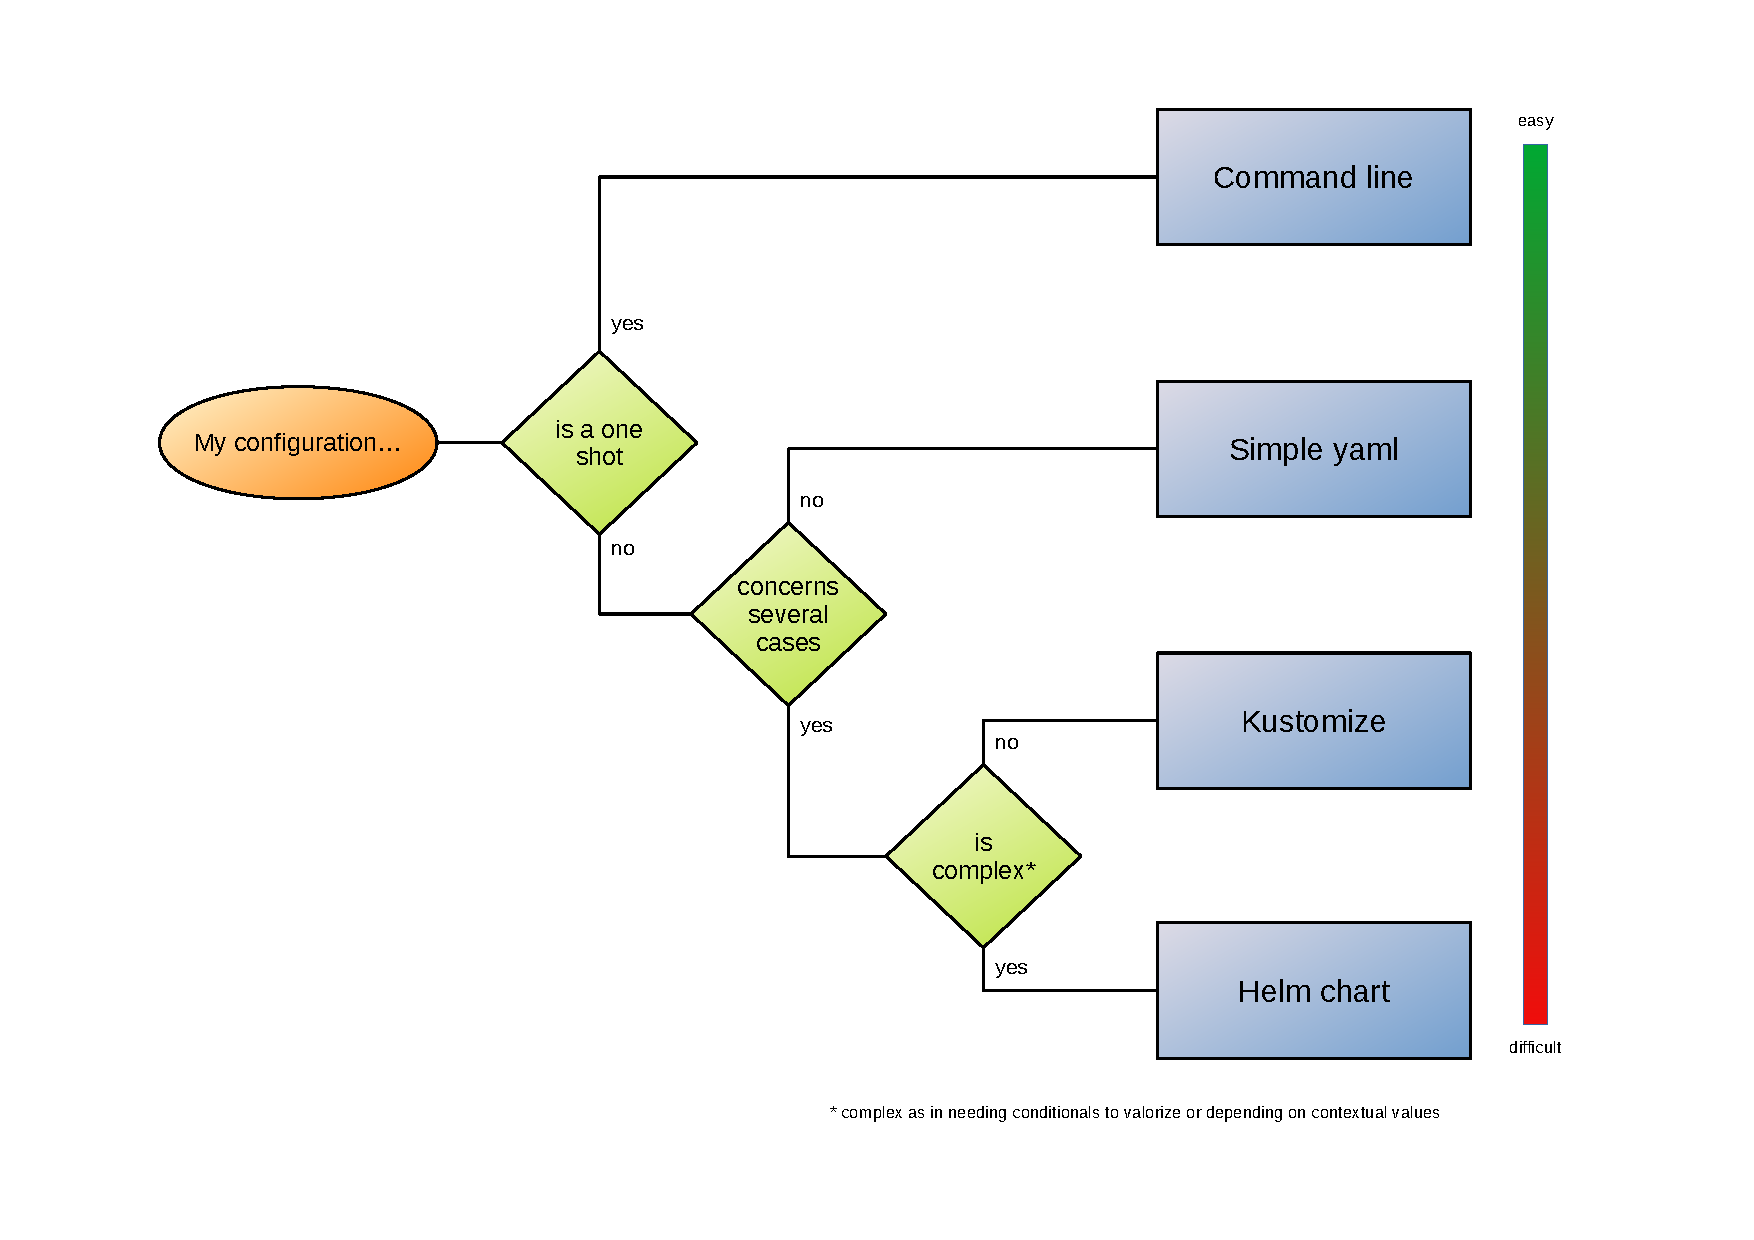
\includegraphics[height=7.5cm]{../../../resources/color/choiceConfigKind.pdf}
		\end{center}
	\end{frame}
	
	\begin{frame}
		\frametitle{Layer based configuration}
		
		Kustomize is a tool now integrated in kubectl.
		
		\bigskip
		It manage the configuration using a layer based system.
		
		That means that a configuration is the result of a base configuration, on wich layers are applyed.
		
		Eache layer can contains new resources or new patches.
		
		\bigskip
		As a base layer is considered as a resource, that enable to define a configuration as the concatenation of several other configurations and their patches.
	\end{frame}
	
	\begin{frame}[fragile]
		\frametitle{Initialize the base}
		
		We are creating a folder tree to sort our files
		\begin{block}{Command line 1}
			\begin{verbatim}
				mkdir kube-kusto-conf
				cd kube-kusto-conf
				mkdir base
				cd base
			\end{verbatim}
		\end{block}
	\end{frame}
	
	\begin{frame}[fragile]
		\frametitle{Initialize the base}
		
		We are using our previous deployment.yaml as starting point
		\begin{block}{Command line 1}
			\begin{verbatim}
				cp ../../deployment.yaml .
				touch kustomization.yaml
				kustomize edit fix
				kustomize edit add resource deployment.yaml
				kustomize build
				kubectl apply -k .
			\end{verbatim}
		\end{block}
	\end{frame}
	
	\begin{frame}[fragile]
		\frametitle{Add a parameter to our worker}
		
		Modify the worker to use a parameter:
		\begin{block}{worker.sh}
			\begin{verbatim}
				while true; do
				  echo "I'm $NAME and it is $(date)"
				  sleep 2
				done
			\end{verbatim}
		\end{block}
	\end{frame}
	
	\begin{frame}[fragile]
		\frametitle{Deploy the new version in our cluster}
		
		First we need to create a new version of the image:
		\begin{block}{Command line 1}
			\begin{verbatim}
				docker build -t <registry>/training/worker-<id>:v2 \
				                ../../
				docker push <registry>/training/worker-<id>:v2
			\end{verbatim}
		\end{block}
	\end{frame}
	
	\begin{frame}[fragile]
		\frametitle{Deploy the new version in our cluster}
		
		Change the deployment configuration:
		\begin{block}{deployment.yaml}
			Replace v1 by v2
			
			Add to the container part:
			\begin{verbatim}
				env:
				- name: NAME
				  value: <myName>
			\end{verbatim}
		\end{block}
		
		And finaly apply the modification:
		\begin{block}{Command line 1}
			\begin{verbatim}
				kubectl apply -k .
			\end{verbatim}
		\end{block}
	\end{frame}
	
	\begin{frame}
		\frametitle{Deploy the new version in our cluster}
		
		There are too many operations.
		
		\bigskip
		Is there a way to simplify this?
	\end{frame}